\documentclass[a4paper,12pt,french]{report}

%====================== PACKAGES ======================
\usepackage{multirow}
%\usepackage[french]{babel}
\usepackage[utf8x]{inputenc}
%pour gérer les positionnement d'images
\usepackage{float}
\usepackage{amsmath}
\usepackage{graphicx}
%\usepackage[colorinlistoftodos]{todonotes}
\usepackage{url}
%pour les informations sur un document compilé en PDF et les liens externes / internes
\usepackage{hyperref}
%pour la mise en page des tableaux
\usepackage{array}
\usepackage{tabularx}
\usepackage{enumitem}
%pour utiliser \floatbarrier
%\usepackage{placeins}
%\usepackage{floatrow}
%espacement entre les lignes
\usepackage{setspace}
%modifier la mise en page de l'abstract
\usepackage{abstract}
%police et mise en page (marges) du document
%\usepackage[T1]{fontenc}
\usepackage[top=2cm, bottom=2cm, left=2cm, right=2cm]{geometry}
%Pour les galerie d'images
\usepackage{subfig}

\usepackage{indentfirst}
\usepackage{algorithm}
\usepackage{algpseudocode}
\usepackage{longtable}
\usepackage[Glenn]{fncychap}
\ChNameUpperCase
\ChNumVar{\fontsize{40}{42}\usefont{OT1}{ptm}{m}{n}\selectfont}
\ChTitleVar{\Large}
%pour l'ajout de la table des matières dans la table des matières ndam njoya
\usepackage{tocbibind} 
\usepackage{color}
\usepackage[french]{babel}
%====================== INFORMATION ET REGLES ======================

%rajouter les numérotation pour les \paragraphe et \subparagraphe
\setcounter{secnumdepth}{4}
\setcounter{tocdepth}{4}
\hypersetup{                            % Information sur le document
pdfauthor = {Mohamed el bachir},          % Auteurs
pdftitle = {Memoire - Deep Analysis and prediction of chikungunya using ensemble regression tools},           % Titre du document
pdfsubject = {Mémoire},       % Sujet
pdfstartview={FitW},                    % ajuste la page à la largueur de l'écran
hidelinks}                              % désactive les cadres autour des liens
%pdfcreator = {MikTeX},% Logiciel qui a créé le document
%pdfproducer = {}} % Société qui produit le logiciel

%======================== DEBUT DU DOCUMENT ========================

\begin{document}

% régler l'espacement entre les lignes
\newcommand{\HRule}{\rule{\linewidth}{0.5mm}}

% page de garde
\begin{titlepage}
\begin{center}
\begin{minipage}{0.38\textwidth}
\begin{centering} 
\bf{UNIVERSITÉ DE NGAOUNDÉRÉ}\\[0.2cm]
\bf{FACULTÉ DES SCIENCES}\\[0.2cm]
\bf{DÉPARTEMENT DE MATHEMATIQUES ET INFORMATIQUE}\\[0.2cm]
\end{centering}
\end{minipage}
\begin{minipage}{0.20\textwidth}
	\centering
	
\includegraphics[width=0.30\textwidth]{./LogoUnivNg}\\
	
\includegraphics[width=0.30\textwidth]{./LogoUnivNgFS}
	
\end{minipage}
\begin{minipage}{0.38\textwidth}
\begin{centering} 
\bf{THE UNIVERSITY OF NGAOUNDERE}\\[0.2cm]
\bf{FACULTY OF SCIENCE}\\[0.2cm]
\bf{DEPARTMENT OF MATHEMATICS AND COMPUTER SCIENCE}\\[0.2cm]
\end{centering}
\end{minipage}\\[1.5cm]

\begin{center}
	\textbf{ÉCOLE DOCTORALE : SCIENCES, TECHNOLOGIE ET INGÉNIERIE (STI)}\\[.09cm]
	\textbf{UFD : MATHÉMATIQUES, INFORMATIQUE, INGÉNIERIE ET APPLICATION (M2IAP)}	
\end{center}
%\begin{tabularx}{\textwidth}{XcX}
%	\raggedright\bfseries{UNIVERSITÉ DE NGAOUNDÉRÉ} & & \raggedleft\bfseries{THE UNIVERSITY OF NGAOUNDERE} \\[0.2cm]
%	\raggedright\bfseries\itshape{FACULTÉ DES SCIENCES} & & \raggedleft\bfseries\itshape{FACULTY OF SCIENCE} \\[0.2cm]
%	\raggedright\itshape{DÉPARTEMENT DE MATHEMATIQUES ET INFORMATIQUE} & & \raggedleft\itshape{DEPARTMENT OF MATHEMATICS AND COMPUTER SCIENCE} \\[0.5cm]
%	& \begin{minipage}{1cm}\centering
\includegraphics[width=0.10\textwidth]{./LogoUnivNg}\\
\includegraphics[width=0.10\textwidth]{./LogoUnivNgFS}\end{minipage} & \\[0.5cm]
%\end{tabularx}



% Upper part of the page. The '~' is needed because only works if a paragraph has started.
%
\includegraphics[width=0.10\textwidth]{./LogoUnivNg}~\\[0.8cm]
%
\includegraphics[width=0.10\textwidth]{./LogoUnivNgFS}~\\[0.8cm]
%
\includegraphics[width=0.35\textwidth]{./LogoUnivNgFS}~\\[1cm]


%\sf{\large \textbf{Unité de Formation Doctorale Mathématiques, Informatique et Applications}}\\[0.2cm]
%\sf{\large   \textbf{\textit{Doctoral Training Unit in Mathematics, Computer Science and Applications}}}\\[0.8cm]

%\textsc{\Large }\\[0.5cm]

% Title \color{blue}{}
\makebox[\linewidth]{\rule{\textwidth}{0.5pt}}
\begin{center}
	\textbf{\textsc{\color{blue}{ANALYSE APPROFONDIE ET PRÉDICTION DU CHIKUNGUNYA À L'AIDE D'UNE APPROCHE DE RÉGRESSION D'ENSEMBLE\\}}}
\end{center}
\makebox[\linewidth]{\rule{\textwidth}{0.5pt}}

\vfill
\begin{center}
	\textbf{\large{Mémoire}} \\[0.2cm]
	\vspace{0.01cm}
	\textbf{\large{Présenté en vue de l'obtention du diplôme de} }\\[0.2cm]
	\textbf{\large{Master en Systèmes et Logiciels en Environnements Distribués}}\\[0.2cm]
	\textbf{\large{Par}}:\\[0.2cm]
	\begin{large}
		\textbf{MOHAMED EL BACHIR BOUBA NGANADAKOUA}\\[0.2cm]
		{\large (Licence en Informatique)}\\[0.2cm]
	\end{large}
	\begin{normalsize}
		\vspace{0.1cm}
		{\large Matricule} : \textbf{{\large 19A666FS}}\\
		%\vspace{0.5cm}
	\end{normalsize}
\end{center}
\vfill
\rule{\textwidth}{1pt}
\begin{center}
		\textbf{\large{Soutenu le 26 septembre 2024 devant un jury composé de :}} \\[0.2cm]
		\textbf{Président}: Pr Ndam NJOYA AROUNA, Maître de conférences \\[0.2cm]
		\textbf{Rapporteur}: Dr Abboubakar HAMADJAM , Chargé de cours , IUT, Université de Ngaoundéré \\[0.2cm]
		\textbf{Examinateur}: Dr Rodrigue SAOUNGOUMI SOURPELE , Chargé de cours\\[0.2cm]
\end{center}
\vfill
%\rule{\textwidth}{1pt}
%{\textbf{Sous la direction de}}:\\[0.5cm]
%\begin{tabularx}{\textwidth}{lXr}
%	\sc{Dr. ABBOUBAKAR Hamadjam} & & \sc{Dr. ZONGO MEYO Epse NDO} \\[0.2cm]
%	Chargé de Cours &  &  Chargé de Cours\\[0.2cm]
%	Institut Universitaire de Technologie & & Faculté des sciences \\[0.2cm]
%	Université de Ngaoundéré & & Université de Ngaoundéré \\[0.2cm]
%\end{tabularx}
%\vspace{0.4cm}
%\rule{\textwidth}{0.5pt}

%Université de Ngaoundéré
% Author and supervisor
%\begin{minipage}{0.1\textwidth}
%\begin{flushleft} \large
%\emph{Auteur:}\\
%Premier \textsc{Auteur}\\
%Deuxième \textsc{Auteur}\\
%Troisième \textsc{Auteur}\\
%Quatrième \textsc{Auteur}
%\end{flushleft}
%\end{minipage}
%\begin{minipage}{0.1\textwidth}
%\begin{flushright} \large
%\emph{Client:} \\
%Prénom \textsc{Nom}\\
%\emph{Référent:} \\
%Prénom \textsc{Nom}
%\end{flushright}
%\end{minipage}


% Bottom of the page
%{\large \today}
{\large \bf{Année académique 2023 - 2024}}

\end{center}
\end{titlepage}

% page blanche
%\newpage % ndam njoya
%~
% ne pas numéroter cette page
%\thispagestyle{empty} % ndam njoya

\pagenumbering{roman} \setcounter{page}{1}
%\newpage % ndam njoya

\begin{spacing}{1.5}

\chapter*{Dédicace}
\addcontentsline{toc}{chapter}{Dédicace}

\renewcommand{\abstractnamefont}{\normalfont\Large\bfseries}
%\renewcommand{\abstracttextfont}{\normalfont\Huge}


\hskip7mm
\begin{spacing}{1.3}
	\hspace{13cm}\Large{À}
	\begin{flushright}
	\itshape
mon père BOUBA Nana Dekwa,\\
ma mère ABIBA Kouyessi,\\
mes sœurs.\\
	\end{flushright}
\end{spacing}


\chapter*{Remerciements}
\addcontentsline{toc}{chapter}{Remerciements}

\renewcommand{\abstractnamefont}{\normalfont\Large\bfseries}
%\renewcommand{\abstracttextfont}{\normalfont\Huge}


\hskip7mm
\begin{spacing}{1.3}
Nous exprimons notre profonde gratitude à Allah le Tout-Puissant, source d’inspiration et de force, qui a rendu possible l’accomplissement de ce travail. Nos remerciements les plus sincères vont à l’endroit de : 
\begin{itemize}
	\item Monsieur le Doyen de la Faculté des Sciences de l’Université de Ngaoundéré, pour la qualité de l’enseignement dispensé ;
    \item Pr. Dr. Ing DAYANG PAUL, Chef du Département de Mathématiques et Informatique de la Faculté des Sciences de l’Université de Ngaoundéré ;
    \item Mon directeur de mémoire, Dr. ABBOUBAKAR Hamadjam, Chargé de Cours à l’Université de Ngaoundéré, au Département de Génie Informatique à l’Institut Universitaire de Technologie, pour m'avoir proposé ce sujet de recherche et pour ses précieux conseils ;
    \item Mon Co-directeur Dr. ZONGO MEYO Epse NDO pour son soutien; 
    \item Les enseignants du Département de Mathématiques et Informatique de la Faculté des Sciences de l’Université de Ngaoundéré, ainsi que les membres du jury, pour avoir accepté d'examiner ce travail ;
    \item À ma famille, pour leurs précieux conseils, leur soutien indéfectible et leurs encouragements constants tout au long de mes études ;
    \item À mon oncle ABDEL FADEL LIMAKAMATA pour son soutien et son encouragement ;
    \item À ma grande sœur ELHAM BOUNOU MIJILEKOUA et son ami AISSATOU BIRI qui m'a toujours considéré comme son petit frère et m'a toujours soutenu.   
    \item Mes camarades de promotion, pour la convivialité, le partage de connaissances et l'entraide dont nous avons bénéficié ensemble.
\end{itemize}

À tous, un grand merci.
\end{spacing}


\addtocontents{toc}{\protect\setcounter{tocdepth}{-1}}
\tableofcontents
\addtocontents{toc}{\protect\setcounter{tocdepth}{2}}
%\thispagestyle{empty}
%\setcounter{page}{0}
% ne pas numéroter le sommaire

\renewcommand\listfigurename{Liste de figures}
\listoffigures % ndam njoya

\renewcommand\listfigurename{List of tables}
\listoftables % ndam njoya

\newpage
\chapter*{Notation et abr\'{e}viations}
\addcontentsline{toc}{chapter}{Notation et abr\'{e}viations}
\renewcommand{\abstractnamefont}{\normalfont\Large\bfseries}
%\renewcommand{\abstracttextfont}{\normalfont\Huge}
%\chapter*{}
%\addcontentsline{toc}{chapter}{Notation et abbr�viations}

\hskip7mm
\begin{spacing}{1.3}
	
	\begin{tabular}{ll}
		
		\textbf{CHIKV} & Chikungunya virus\\
		\textbf{WHO} & World Health Organization\\
		\textbf{PAHO} &  Pan American Health Organization\\
		\textbf{OMS} & Organisation Mondiale de la Sante\\
		\textbf{CDC} & Centers for Disease Control and Prevention\\
		\textbf{\textit{Ae}} & Aedes\\
		%\textbf{BCO} & Bee Colony Optimization : Algorithmes de colonie d�abeilles\\
		
	\end{tabular}
\end{spacing}

\chapter*{Résumé}
\addcontentsline{toc}{chapter}{Résumé}

\renewcommand{\abstractnamefont}{\normalfont\Large\bfseries}
%\renewcommand{\abstracttextfont}{\normalfont\Huge}

%\begin{abstract}
\hskip7mm

\begin{spacing}{1.3}

\end{spacing}

Le virus du chikungunya, transmis principalement par les moustiques \textbf{Aedes aegypti} et \textbf{Aedes albopictus}, représente une menace croissante pour la santé publique mondiale en raison de sa propagation rapide et de ses effets débilitants. Récemment, des épidémies ont été signalées non seulement en Afrique centrale et orientale, mais aussi en Amérique du Sud et en Asie du Sud-Est. Prédire ces épidémies reste un défi majeur en raison de l'interaction complexe entre les facteurs environnementaux, climatiques et biologiques. Les approches traditionnelles de surveillance épidémiologique se révèlent souvent insuffisantes pour anticiper les épidémies de manière proactive.

Cette recherche se concentre sur le \textbf{Tchad}, le \textbf{Brésil}, et le \textbf{Paraguay}, trois pays où le chikungunya a émergé comme un problème significatif de santé publique. En raison de la disponibilité limitée de données au Tchad, des données supplémentaires provenant du Brésil et du Paraguay sont intégrées pour renforcer l'analyse. Le but de cette thèse est de développer et d'évaluer des modèles prédictifs pour les épidémies de chikungunya en utilisant des techniques avancées d'apprentissage automatique, en particulier la régression d'ensemble.

Les modèles choisis pour cette étude incluent le \textbf{Random Forest Regressor}, le \textbf{XGBoost Regressor} optimisé via \textbf{Grid Search}, ainsi qu'un modèle d'ensemble (\textbf{Voting Regressor}) combinant \textbf{Linear Regression}, \textbf{Decision Tree Regressor}, et le \textbf{XGBoost Regressor} optimisé. Ces modèles seront formés et validés à partir de données épidémiologiques et climatiques.

Cette thèse commence par une analyse approfondie de l'épidémiologie du chikungunya et de ses dynamiques de transmission, suivie d'une revue des applications actuelles de l'intelligence artificielle dans la prédiction des maladies. Les modèles sont ensuite testés et évalués sur la base de critères de performance tels que la sensibilité, la spécificité, et la valeur prédictive.

Les résultats de cette recherche montrent l'efficacité des techniques de régression d'ensemble pour améliorer la précision des prévisions épidémiologiques, et offrent des perspectives nouvelles pour l'intervention en santé publique dans les régions affectées.

\textbf{Mots-clés} : \textit{Chikungunya, Régression d'ensemble, Random Forest, XGBoost, Apprentissage Automatique, Données Climatiques, Prévision Épidémiologique}

%\end{abstract}

\chapter*{Abstract}
\addcontentsline{toc}{chapter}{Abstract}

\renewcommand{\abstractnamefont}{\normalfont\Large\bfseries}
%\renewcommand{\abstracttextfont}{\normalfont\Huge}

%\begin{abstract}
\hskip7mm
%

\begin{spacing}{1.3}
	
The chikungunya virus, transmitted mainly by the mosquitoes \textbf{Aedes aegypti} and \textbf{Aedes albopictus}, represents a growing threat to global public health due to its rapid spread and debilitating effects. Recently, epidemics have been reported not only in Central and East Africa, but also in South America and Southeast Asia. Predicting these epidemics remains a major challenge due to the complex interplay between environmental, climatic and biological factors. Traditional epidemiological surveillance approaches often prove insufficient to proactively anticipate epidemics.

This research focuses on \textbf{Chad}, \textbf{Brazil}, and \textbf{Paraguay}, three countries where chikungunya has emerged as a significant public health problem. Due to limited data availability in Chad, additional data from Brazil and Paraguay are incorporated to strengthen the analysis. The aim of this thesis is to develop and evaluate predictive models for chikungunya epidemics using advanced machine learning techniques, in particular ensemble regression.

The models chosen for this study include the \textbf{Random Forest Regressor}, the \textbf{XGBoost Regressor} optimized via \textbf{Grid Search}, as well as an ensemble model (\textbf{Voting Regressor}) combining \textbf{Linear Regression}, \textbf{Decision Tree Regressor}, and the optimized \textbf{XGBoost Regressor}. These models will be trained and validated using epidemiological and climatic data.

This thesis begins with an in-depth analysis of the epidemiology of chikungunya and its transmission dynamics, followed by a review of current applications of artificial intelligence in disease prediction. The models are then tested and evaluated on the basis of performance criteria such as sensitivity, specificity and predictive value.

The results of this research demonstrate the effectiveness of ensemble regression techniques in improving the accuracy of epidemiological forecasts, and offer new perspectives for public health intervention in affected regions.

\textbf{Keywords} : \textit{Chikungunya, Ensemble regression, Random Forest, XGBoost, Machine learning, Climatic data, Epidemiological forecast}

%\textbf{Keywords:} \textit{Machine learning, AI.}
\end{spacing}
%\end{abstract}


\newpage

% espacement entre les lignes d'un tableau
\renewcommand{\arraystretch}{1.5}

%====================== INCLUSION DES PARTIES ======================

\thispagestyle{empty}
% recommencer la numérotation des pages à "1"
\pagenumbering{arabic} % ndam njoya 
\setcounter{page}{1}
\newpage

\chapter*{Introduction Générale}
\addcontentsline{toc}{chapter}{Introduction Générale} 
Le chikungunya est une maladie virale transmise à l'homme par des moustiques infectés par le virus du chikungunya. Les moustiques impliqués dans la transmission sont \textit{Aedes aegypti} et \textit{Aedes albopictus}~\cite{intro}. Le 2 août 2024, le Centre européen de contrôle et de prévention des maladies (ECDC) a indiqué qu'environ \textbf{350 000} cas de maladie à virus chikungunya (CHIKVD) et plus de \textbf{140 décès} ont été signalés dans le monde en 2024, Ces cas proviennent de 21 pays d'Amérique, d'Asie, d'Afrique et d'Europe~\cite{chikvecdc}. Le chikungunya se manifeste par des symptômes tels que \textbf{fièvre}, \textbf{douleurs articulaires}, \textbf{maux de tête}, \textbf{douleurs musculaires}, \textbf{gonflements articulaires}, et \textbf{éruptions cutanées}. Bien que les décès dus au chikungunya soient \textbf{rares}, le virus peut provoquer de graves complications, en particulier chez les personnes âgées ou celles souffrant de \textit{maladies chroniques}. Une détection précoce est cruciale pour prévenir la propagation de la maladie.

L'objectif de ce mémoire est de développer un modèle prédictif du chikungunya, en utilisant des approches de régression d'ensemble issues de l'intelligence artificielle. Compte tenu du manque de données suffisantes pour le \textbf{Tchad}, nous avons étendu notre étude aux données du \textbf{Brésil} et du \textbf{Paraguay}, où des cas de chikungunya ont également été signalés. Cette approche nous permet de tirer parti d'un ensemble de données plus vaste et diversifié pour améliorer la précision de nos prévisions.

Nous nous posons donc la question suivante : comment utiliser les techniques d'apprentissage automatique, en particulier l'approche ensembliste, pour prédire et analyser les épidémies de chikungunya ?

Les objectifs spécifiques de ce travail sont les suivants :
\begin{itemize}
	\item Comprendre les concepts liés au chikungunya à la régression d'ensemble;
	\item Prédire les épidémies de chikungunya en se basant sur les données climatiques et les cas rapportés au Tchad, au Brésil, et au Paraguay ;
\end{itemize}

Le reste du document est structuré comme suit : le premier chapitre est dédié à l'épidémiologie du chikungunya avec un accent particulier sur les cas au Tchad, au Brésil , au Paraguay et une vue bref sur le plan national. Le deuxième chapitre introduit les concepts de base sur les méthodes d'ensemble de régression. Le troisième chapitre présente la conception générale et détaillée du modèle proposé. Dans le quatrième chapitre, nous illustrons l'efficacité de notre modèle à travers des résultats de simulation. Enfin, le mémoire se conclut par une synthèse des résultats et des perspectives pour des recherches futures.



\chapter{Épidémiologie de la Chikungunya}

\section{Origine de la Chikungunya}
La fièvre \textbf{Chikungunya} est une maladie virale décrite pour la première fois en \textbf{1952} lors d'une épidémie dans le sud de la \textbf{Tanzanie}. Le nom vient d'un mot de la langue \textit{Makonde}, parlée dans le sud-est de la Tanzanie et le nord du Mozambique, qui signifie "\textit{devenir contorsionné}"\footnote{Le terme "contorsionné" fait référence à la posture courbée et aux douleurs articulaires intenses souvent associées à la maladie.} ou "\textit{ce qui se plie}". Le virus a été isolé pour la première fois en Thaïlande en 1958.\cite{origin}

\section*{Évolution géographique et épidémiologique}
En \textbf{avril 2005}, il a été confirmé que le CHIKV était à l'origine d'une épidémie de maladie ressemblant à la dengue sur les îles Comores, situées au large de la côte est du Mozambique septentrional ; il s'agissait de la première émergence connue du CHIKV dans la région du sud-ouest de l'océan Indien. En raison de similitudes cliniques, cette épidémie a d'abord été suspectée d'être causée par le virus de la dengue, soulignant le fait que la maladie CHIKV est souvent mal diagnostiquée et que le nombre réel de cas dans une région donnée peut être sous-estimé. Peu après, les premiers cas de CHIKV ont été signalés à Mayotte, à Maurice et sur l'île française de La Réunion. Le nombre de cas dans ces régions a rapidement augmenté, notamment en raison de taux d'attaque atteignant \textbf{35\%} à \textbf{75\%}. À la fin de l'année \textbf{2005}, après une période apparente d'environ 32 ans pendant laquelle le CHIKV n'a pas été détecté, l'Inde a signalé des cas de maladie à CHIKV dans de nombreux États, le nombre officiel de cas suspects atteignant finalement plus de 1,3 million. L'épidémie de CHIKV a continué à se propager, provoquant d'importantes flambées au Sri Lanka et dans de nombreux autres pays d'Asie du Sud-Est. Au cours de cette épidémie, le CHIKV a été introduit dans des pays où il n'est pas endémique par des voyageurs virémiques\footnote{ Organisme hébergeant un virus et pouvant en être le vecteur}, et la transmission autochtone du CHIKV a été observée pour la première fois dans de nombreux pays, dont l'Italie, la France, la Nouvelle-Calédonie, la Papouasie-Nouvelle-Guinée, le Bhoutan et le Yémen. La propagation rapide et explosive du CHIKV a incité l'Organisation panaméricaine de la santé (OPS) et les Centers for Disease Control and Prevention (CDC) à publier un guide de préparation qui prévoyait de futures épidémies potentielles de CHIKV dans les Amériques. Cette prédiction s'est maintenant concrétisée, puisqu'en décembre 2013, l'Organisation mondiale de la santé (OMS) a signalé la première transmission locale du CHIKV dans l'hémisphère occidental, sur l'île caribéenne de Saint-Martin. Le 18 juillet 2014, le CHIKV avait provoqué plus de \textbf{440 000 cas} de maladie dans plus de 20 pays des Caraïbes, d'Amérique centrale et d'Amérique du Sud (voir figure \ref{fig:chikvwestern}). En outre, les CDC ont signalé plus de 230 cas importés d'infection à CHIKV sur le territoire continental des États-Unis, ainsi que des cas acquis localement en Floride. Ainsi, en moins de 10 ans, le CHIKV s'est propagé depuis les côtes du Kenya dans l'océan Indien, le Pacifique et les Caraïbes, provoquant des millions de cas de maladie dans plus de 50 pays. En d'autres termes, le CHIKV est redevenu un véritable agent pathogène mondial~\cite{Peyrefitte2007}.
\begin{figure}[!h]
	\begin{center}
		%taille de l'image en largeur
		%remplacer "width" par "height" pour régler la hauteur
		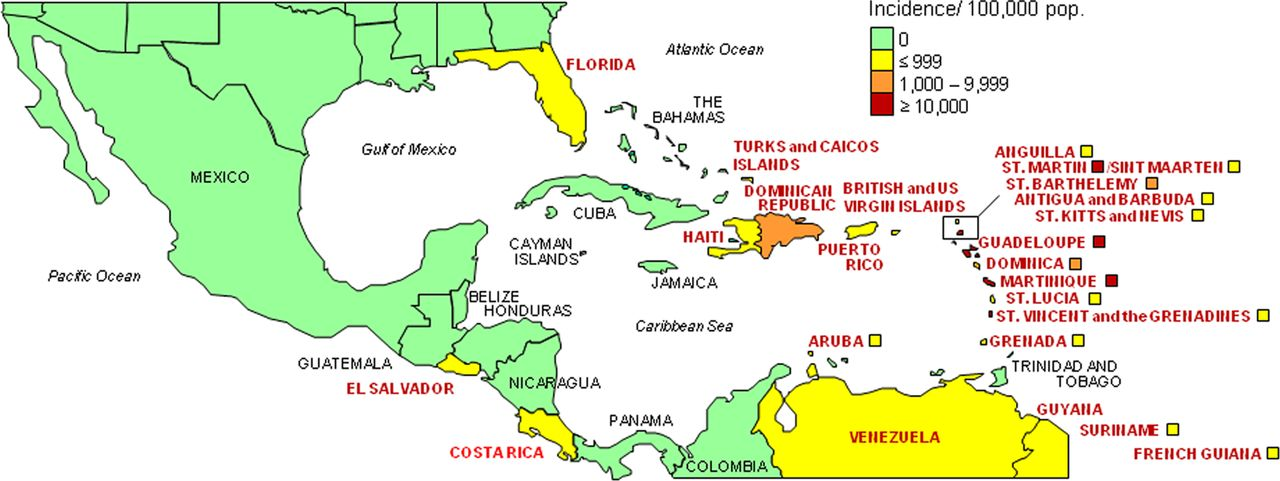
\includegraphics[width=14cm]{images/zjv9990995820001}
	\end{center}
	%légende de l'image
	\caption{CHIKV dans l'hémisphère occidental\cite{Peyrefitte2007}.}
	\label{fig:chikvwestern}
\end{figure}

\section{Agent Pathogène}
Le virus du chikungunya (CHIKV), un alphavirus transmis par les moustiques, dont le génome est constitué d'un ARN monocaténaire à sens positif de $\sim$12 kb~\cite{JournalofVirology}. La figure (\ref{fig:chikv}) montre une image microscopique du virus du chikungunya
\begin{figure}[!h]
	\begin{center}
		%taille de l'image en largeur
		%remplacer "width" par "height" pour régler la hauteur
		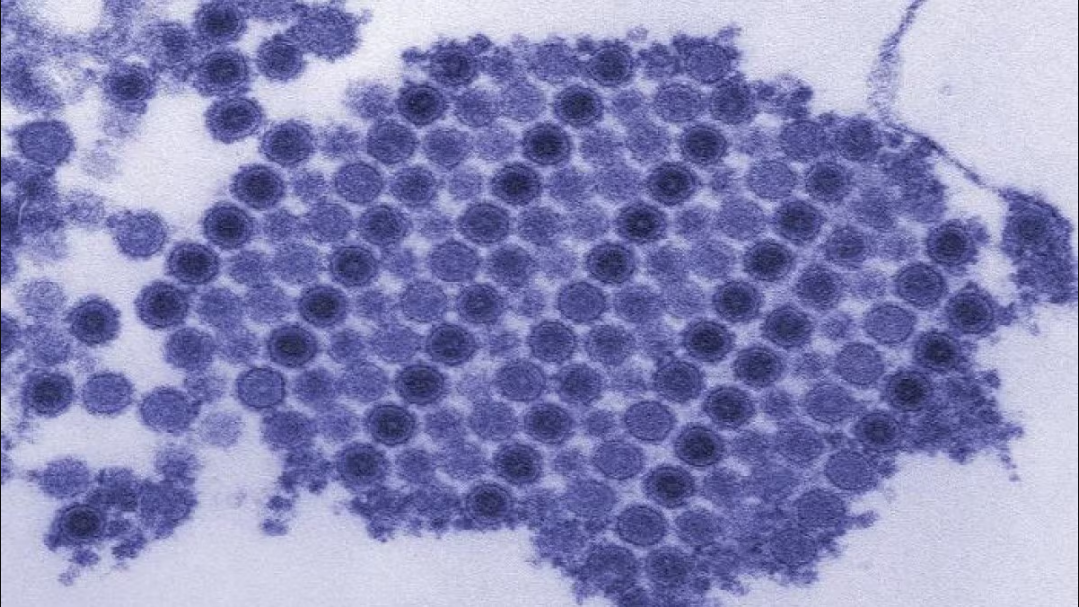
\includegraphics[width=12cm]{images/CHIK_17550_TEM}
	\end{center}
	%légende de l'image
	\caption{Image au microscope électronique du virus du chikungunya~\cite{chikvcdc}}
	\label{fig:chikv} 
\end{figure}

\section{Mode de Transmission}
Comprendre les mécanismes de transmission du virus chikungunya est essentiel pour développer des stratégies de prévention efficaces. Cette section examine les principaux vecteurs de la maladie, les conditions environnementales qui favorisent la propagation du virus et les dynamiques de transmission entre les hôtes humains et animaux.
\subsection{Vecteurs : Les moustiques \textit{Aedes}}
Le virus du chikungunya est un \textbf{alphavirus}, similaire aux virus de Mayaro et de Ross River, appartenant à la famille \textit{Togaviridae}, au genre \textit{Alphavirus}. Le virus du chikungunya est principalement transmis à l'homme par la piqûre d'un moustique infecté, principalement \textit{Aedes aegypti} (Voir Figure \ref{fig:aedes}) et \textit{Ae. albopictus}~\cite{chikvcdc}.
\begin{figure}[!h]
	\begin{center}
		%taille de l'image en largeur
		%remplacer "width" par "height" pour régler la hauteur
		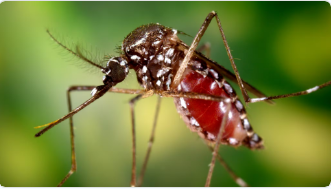
\includegraphics[width=10cm]{images/moustique}
	\end{center}
	%légende de l'image
	\caption{Le moustique \textit{Aedes aegypti }plein de sang~\cite{chikvcdc}}
	\label{fig:aedes}
\end{figure} 

\subsection{La transmission}
Le \textbf{CHIKV} se transmet selon deux cycles différents :
\begin{itemize}
	\item \textbf{Cycle urbain} : transmission de l'homme au moustique.
	\item \textbf{Cycle sylvatique} : transmission de l'animal au moustique, puis à l'homme.
\end{itemize}
Le cycle sylvatique est la principale forme de transmission en \textbf{Afrique}. Ailleurs, dans les zones plus densément peuplées, le CHIKV se maintient principalement dans un cycle urbain, dans lequel les humains sont les principaux hôtes et les moustiques du genre \textit{Aedes} les vecteurs (voir figure\ref{fig:chikvtransmission}).
bien que \textit{Ae. aegypti} continue d'être un vecteur viral important, comme on l'a vu lors de la flambée épidémique dans les Caraïbes en 2013. La transmission verticale de la mère à l'enfant a été postulée pour expliquer les incidences postérieures à 2005 , étant particulièrement délétère lorsque la mère est infectée jusqu'à quatre jours après l'accouchement, bien que cette hypothèse ait été contestée \cite{ganesan2017chikungunya}.

\begin{figure}[!h]
	\begin{center}
		%taille de l'image en largeur
		%remplacer "width" par "height" pour régler la hauteur
		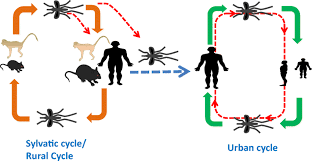
\includegraphics[height=8cm]{images/trans}
	\end{center}
	%légende de l'image
	\caption{mode de transmission du Chikungunya~\cite{infographicCHIKV}.}
	\label{fig:chikvtransmission}
\end{figure}
\section{Symptômes et Diagnostic}
La reconnaissance des symptômes et l'établissement d'un diagnostic précis sont essentiels pour la gestion efficace des cas de chikungunya. Cette section examine les manifestations cliniques typiques de l'infection par le virus chikungunya ainsi que les méthodes diagnostiques utilisées pour identifier la maladie.
\subsection{Symptômes}
Chez les patients symptomatiques, la maladie se déclare généralement \textbf{4 à 8 jours} après la \textbf{piqûre} d'un\textbf{ moustique infecté}. Elle se caractérise par une brusque \textbf{poussée de fièvre}, souvent accompagnée de \textbf{fortes douleurs articulaires}. Les douleurs articulaires durent généralement quelques jours, mais peuvent être prolongées et durer des semaines, des mois, voire des années. D'autres signes et symptômes courants sont le \textbf{gonflement des articulations}, les \textbf{douleurs musculaires}, les \textbf{maux de tête}, les \textbf{nausées}, la \textbf{fatigue} et les \textbf{éruptions cutanées}. Comme ces symptômes se confondent avec ceux d'autres infections, notamment celles dues aux virus de la dengue et du Zika, les cas peuvent être mal diagnostiqués. En l'absence de douleurs articulaires importantes, les symptômes des personnes infectées sont généralement légers et l'infection peut passer inaperçue.

La plupart des patients se rétablissent complètement de l'infection ; toutefois, des cas occasionnels de complications \textbf{oculaires}, \textbf{cardiaques} et \textbf{neurologiques} ont été signalés dans le cadre d'infections par le \textbf{CHIKV}. Les patients très jeunes et les personnes âgées, sont plus exposés à des formes graves de la maladie. Les nouveau-nés infectés pendant l'accouchement et les personnes âgées souffrant de pathologies sous-jacentes peuvent devenir gravement malades et l'infection par le \textbf{CHIKV} peut augmenter le \textbf{risque de décès}~\cite{origin2}.

Une fois qu'une personne est guérie, les données disponibles suggèrent qu'elle est probablement immunisée contre les infections futures~\cite{auerswald2018broad}.

\subsection{Méthodes de diagnostic}
Le diagnostic peut être retardé en raison de la confusion possible des symptômes avec ceux de la dengue ou du Zika. Les tests \textbf{\textit{immuno-enzymatiques}} (ELISA\footnote{Enzyme-Linked Immunosorbent Assay ( Test de laboratoire couramment utilisé pour détecter des anticorps dans le sang, souvent utilisé pour diagnostiquer des infections. )}) peuvent être utilisés pour confirmer la présence d'anticorps \textbf{anti-CHIKV}, les niveaux d'anticorps IgM\footnote{Immunoglobulin M ( Type d'anticorps produit par le système immunitaire en réponse initiale à une infection. )} étant les plus élevés trois à cinq semaines après l'infection et persistant jusqu'à deux mois. La PCR\footnote{Polymerase Chain Reaction ( Technique de biologie moléculaire utilisée pour amplifier et détecter des séquences d'ADN ou d'ARN spécifiques, permettant d'identifier la présence d'agents pathogènes tels que les virus. )} peut également être utilisée pour génotyper\footnote{déterminer le type ou la variation génétique du virus, en étudiant son matériel génétique (ADN ou ARN).} le virus~\cite{JournalofVirology}.

\section{Méthodes de Contrôle et Traitement}

La gestion efficace de l'épidémie de chikungunya repose sur une combinaison de stratégies de contrôle des vecteurs et d'interventions médicales. Cette section explore les diverses approches utilisées pour prévenir la transmission du virus et traiter les symptômes chez les patients infectés.

\subsection{Méthodes de contrôle}
La prévention de l'infection en évitant les piqûres de moustiques est la \textbf{meilleure protection}. Les patients suspectés d'être infectés par le \textbf{CHIKV} doivent éviter les piqûres de moustiques pendant la première semaine de la maladie afin d'empêcher la transmission aux moustiques, qui peuvent à leur tour infecter d'autres personnes. 

La principale méthode pour réduire la transmission du \textbf{CHIKV} consiste à contrôler les moustiques vecteurs. Pour ce faire, il faut mobiliser les communautés, qui jouent un rôle essentiel dans la réduction des sites de reproduction des moustiques en :

\begin{itemize}
	\item vidant et en nettoyant chaque semaine les récipients contenant de l'eau,
	\item éliminant les déchets,
	\item soutenant les programmes locaux de lutte contre les moustiques.
\end{itemize}

Pendant les épidémies, des insecticides peuvent être :

\begin{itemize}
	\item pulvérisés pour tuer les moustiques adultes volants,
	\item appliqués sur les surfaces à l'intérieur et autour des conteneurs où les moustiques se posent,
	\item utilisés pour traiter l'eau dans les conteneurs afin de tuer les larves immatures.
\end{itemize}

Les autorités sanitaires peuvent également prendre des mesures d'urgence pour contrôler la population de moustiques.

Pour se protéger pendant les épidémies de \textbf{chikungunya}, il est conseillé de :

\begin{itemize}
	\item porter des vêtements qui minimisent l'exposition de la peau aux vecteurs qui piquent pendant la journée,
	\item utiliser des moustiquaires aux fenêtres et aux portes pour empêcher les moustiques de pénétrer dans les maisons,
	\item appliquer des répulsifs sur la peau exposée ou sur les vêtements en respectant scrupuleusement les instructions figurant sur l'étiquette du produit.
\end{itemize}

Les répulsifs doivent contenir du \textbf{DEET}\footnote{DEET, ou N,N-Diethyl-meta-toluamide, est un répulsif chimique largement utilisé pour éloigner les moustiques et autres insectes piqueurs.}, de l'\textbf{IR3535}\footnote{IR3535, ou Ethyl butylacetylaminopropionate, est un répulsif synthétique utilisé contre les moustiques, tiques et autres insectes piqueurs.} ou de l'\textbf{icaridine}\footnote{Icaridine, aussi connue sous le nom de Picaridine, est un répulsif synthétique efficace et moins irritant que le DEET.}~\cite{origin}.


\subsection{Options de traitement}
Le traitement actuel vise à atténuer la gravité des symptômes plutôt qu'à guérir la maladie. Le traitement repose principalement sur l'utilisation d'\textbf{antipyrétiques} et d'\textbf{AINS\footnote{Anti-Inflammatoires Non Stéroïdiens. Ce sont des médicaments utilisés pour réduire l'inflammation, la douleur et la fièvre ( l'ibuprofène, l'aspirine et le naproxène )}}. Cependant, aucune étude n'a évalué systématiquement l'efficacité de ces traitements, et les symptômes peuvent disparaître sans intervention. L'utilisation de \textbf{corticostéroïdes} pour le traitement de la phase aiguë a connu un succès mitigé et est utilisée avec hésitation en raison de la possibilité d'aggravation des symptômes après le traitement. 

Il existe également des preuves émergentes que les médicaments qui entravent le transport du cholestérol, tels que les composés \textbf{amphiphiles cationiques de classe II U18666A} et L'\textbf{imipramine}, peuvent être efficaces contre la fusion membranaire du \textbf{CHIKV}, et ont un potentiel d'action contre d'autres arbovirus\footnote{Arbovirus désigne un virus transmis par des arthropodes, comme les moustiques ou les tiques. Ils incluent des virus responsables de maladies comme la dengue, le Zika, et la fièvre jaune.}.


Pour les arthralgies chroniques graves, des \textbf{antirhumatismaux modificateurs de la maladie (ARMM)}, notamment le \textbf{méthotrexate}, l'\textbf{hydroxychloroquine} ou la \textbf{sulfasalazine}, ont été proposés. Comme pour les traitements aigus, l'efficacité systématique des \textbf{DMARD}\footnote{DMARD, ou Disease-Modifying Antirheumatic Drugs, sont des médicaments qui modifient la progression des maladies inflammatoires chroniques.} pour le traitement chronique est inconnue, bien que des rapports décrivent des résultats positifs avec une cessation des symptômes dans les 4 à 6 mois \cite{ganesan2017chikungunya}.

\newpage

\section{Sur le plan national}
Un cas de virus du chikungunya a été identifié au \textbf{Cameroun} lors d'une épidémie de syndrome de type \textit{dengue} en \textbf{2006}. L'analyse phylogénétique a révélé que ce virus appartient au même groupe que celui circulant en République démocratique du Congo, suggérant la présence continue d'un virus chikungunya génétiquement similaire en Afrique centrale pendant 6 ans~\cite{Peyrefitte2007}.En 2006, plus de \textbf{400} épidémie de type dengue ont été signalés à \textbf{Kumbo} (région du Nord-Ouest du Cameroun). Entre avril et juillet 2006, le \textbf{CHIKV} a été identifié lors d'une épidémie de syndrome fébrile à \textbf{Yaoundé} et \textbf{Douala}. Parallèlement, dans une zone rurale de l'ouest du \textbf{Cameroun}, plusieurs personnes ont également souffert d'un syndrome fébrile aigu. Bien que les investigations aient été menées un an après cette dernière épidémie, les résultats suggèrent une circulation récente du \textbf{CHIKV} dans trois villages de \textbf{Kumbo} (Cameroun occidental). \textbf{Aedes africanus}\footnote{Le \textit{Aedes africanus} est un moustique de la famille des \textit{Aedidae}, souvent trouvé dans les zones de buissons et de raphia. Il est connu pour être un vecteur potentiel du \textit{CHIKV} dans les régions africaines.}~\cite{demanou2010research}. La figure \ref{fig:chikvcameroon} illustrant la zone d'impact dans cette region.
\begin{figure}[h!]
	\centering
	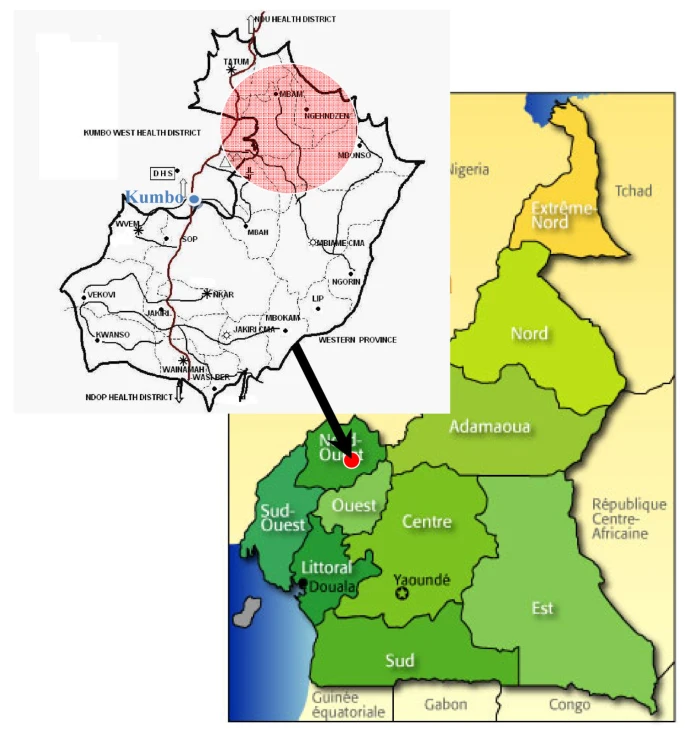
\includegraphics[width=0.7\linewidth]{images/chikvcameroon}
	\caption{zone d'impact du CHIKV dans la region du Nord Ouest~\cite{demanou2010research}}
	\label{fig:chikvcameroon}
\end{figure}


\section{Cas du Tchad}

L'analyse spécifique des cas de chikungunya au Tchad permet de comprendre l'impact de cette maladie dans un contexte régional spécifique. Cette section examine les Points saillants\footnote{Les "points saillants" désignent l'impact du chikungunya}, la mise en contexte du problème dans ce pays d'Afrique central.

%ainsi que les messures prise par l'etat pour la gestion de l'infection par le virus chikungunya dans ce pays d'Afrique centrale.%

\subsection{Point saillants}
le 3 Septembre 2020, \textbf{927} cas ont été notifiés, tous pris en charge en ambulatoire, sans aucun décès. À cette date, le cumul atteignait\textbf{ 13 488} cas, toujours sans décès, avec de nouveaux cas suspects signalés à \textbf{Biltine} et \textbf{Adré} (voir figure \ref{fig:chikvintchadmap}). Le 2 octobre 2020, \textbf{415 cas} ont été notifiés, répartis comme suit : 247 à \textbf{Abéché}, 165 à \textbf{Biltine}, 3 à \textbf{Gozbeida}, et 0 à \textbf{Abdi}, sans aucun décès. à cette date , le cumul atteignait \textbf{34 052 cas}, avec \textbf{un} décès. Tous les patients ont été pris en charge en ambulatoire~\cite{rapport2020oms}.

\begin{figure}[!h]
	\begin{center}
		%taille de l'image en largeur
		%remplacer "width" par "height" pour régler la hauteur
		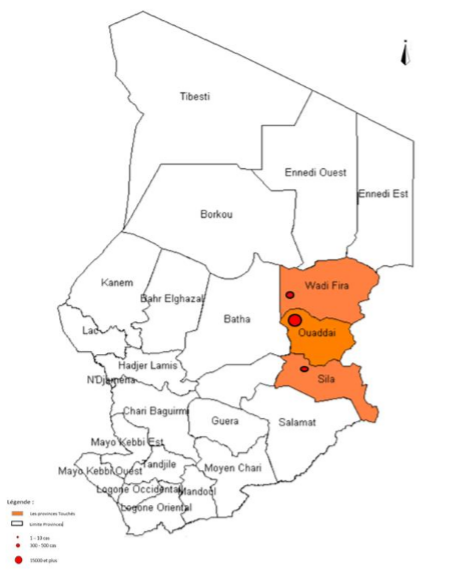
\includegraphics[height=8cm]{images/chadmap}
	\end{center}
	%légende de l'image
	\caption{Region infecté au Tchad~\cite{rapport2020oms}}
	\label{fig:chikvintchadmap}
\end{figure}

\subsection{Contexte}
En \textbf{juillet 2020}, au Tchad, des cas d'une maladie localement appelée \textbf{Kourgnalé}, présentant des symptômes tels que fièvre, céphalées et douleurs articulaires, ont été signalés à Abéché. En août, l'augmentation des cas a conduit à des analyses confirmant la présence du virus Chikungunya le \textbf{12 août 2020}. Entre le 14 août et le 3 septembre dans le rapport de L'OMS, \textbf{13 488} cas ont été enregistrés sans aucun décès~\cite{rapport2020oms}. Les femmes et les personnes âgées de 15 ans et plus étaient les plus touchées. Plus de \textbf{75 \%} des patients présentaient des symptômes graves, et un tiers souffrait d'éruptions cutanées. La figure \ref{fig:cumulcaseschad} présente l'évolution du CHIKV au Tchad .
\begin{figure}[h!]
	\centering
	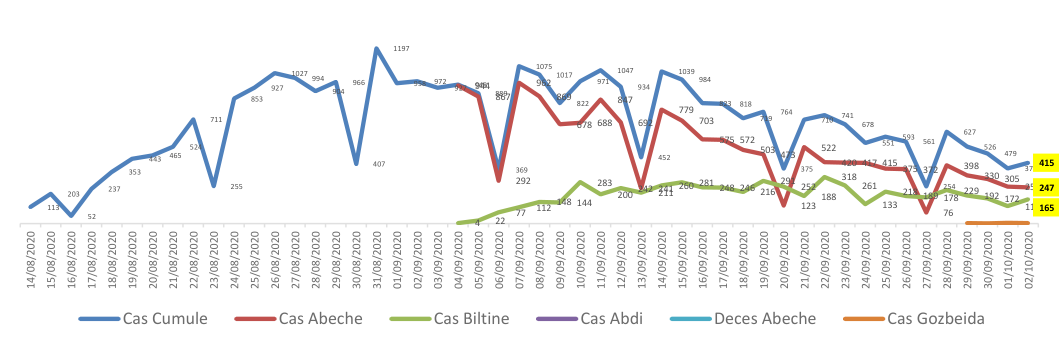
\includegraphics[width=0.9\linewidth]{images/cumul_cases_chad}
	\caption{ Evolution journalière des cas et décès du Chikungunya~\cite{rapport2020oms}}
	\label{fig:cumulcaseschad}
\end{figure}

\section{Cas du Brésil}
Le Brésil est le pays le plus grand et le plus peuplé d'Amérique latine, avec une importante population sensible au CHIKV, ainsi qu'un climat approprié et d'abondantes populations de vecteurs \textit{Ae. aegypti}. Le CHIKV circule localement au Brésil depuis \textbf{2013}, les premiers cas étant principalement limités au \textbf{Nord-Est}.Depuis 2016, le Brésil est l'épicentre des épidémies de chikungunya dans les Amériques avec \textbf{1 659 167} cas, le nombre le plus élevé rapporté dans la région. Contrairement à d'autres pays et territoires des Amériques, le Brésil connaît des épidémies annuelles de chikungunya~\cite{DESOUZA2024100673}.
cette section examine les Points saillant, la mise en contexte du problème dans ce pays.
\subsection{Point saillants}
La figure \ref{fig:brazilregionscases} montre les cas cumulés de chikungunya (c'est-à-dire les cas suspectés et confirmés en laboratoire). Dans les 26 États brésiliens et le district fédéral déclarés au ministère brésilien de la santé entre mars 2013 et juin 2023. (b) Distribution spatio-temporelle des lignées du virus du chikungunya dans les pays et territoires des 26 États brésiliens et du district fédéral. La lignée du chikungunya en circulation a été déterminée sur la base des années pour lesquelles au moins un génome a été séquencé et déposé dans GenBank jusqu'au 17 août 2023. AC = Acre. AL = Alagoas. AM = Amazonas. AP = Amapá. BA = Bahia. CE = Ceará. ES = Espírito Santo. DF = Distrito Federal (district fédéral). GO = Goiás. MA = Maranhão. MG = Minas Gerais. MS = Mato Grosso do Sul. MT = Mato Grosso. PA = Pará. PB = Paraíba. PE = Pernambouc. PI = Piauí. PR = Paraná. RJ = Rio de Janeiro. RN = Rio Grande do Norte. RO = Rondônia. RR = Roraima. RS = Rio Grande do Sul. SC = Santa Catarina. SE = Sergipe. SP = São Paulo. TO = Tocantins. Km = kilomètres. ECSA-American, sous-lignée est-centrale-sud-africaine-américaine~\cite{DESOUZA2024100673}.
\begin{figure}[h!]
	\centering
	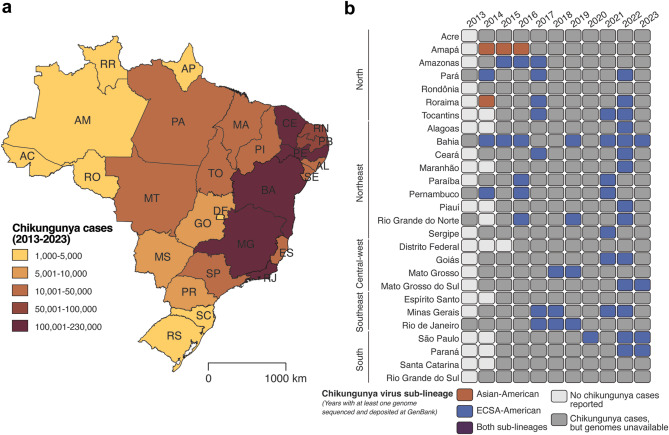
\includegraphics[width=0.9\linewidth]{images/brazil_regions_cases}
	\caption{Épidémiologie et informations génomiques du chikungunya au Brésil.\cite{chikungunya_burden_americas}}
	\label{fig:brazilregionscases}
\end{figure}
\subsection{Contexte}
Le chikungunya a ressurgi en 2022-23 après une période d'accalmie\footnote{Le terme "accalmie" fait référence à une période de calme ou de répit, durant laquelle l'activité ou l'intensité des cas de chikungunya, est réduite.}.le Brésil, notamment dans l'État de Minas Gerais avec \textbf{395} cas pour 100 000 habitants. Depuis son introduction au Brésil en 2014, avec\textbf{ 3,6 millions} de cas signalés à la PAHO/origin, la maladie s'est déplacée du Nord-Est vers le Sud-Est, où en 2023 (voir figure \ref{fig:mapcasesbrazil}), \textbf{30 724 cas} ont été rapportés en seulement 10 semaines, soit deux fois plus qu'en 2022. Le taux de reproduction du virus a atteint des valeurs élevées, entre 1,5 et 2,5, avec des pics en 2018 et 2022~\cite{Ferreira_de_Almeida2023-et}.
\begin{figure}[h!]
	\centering
	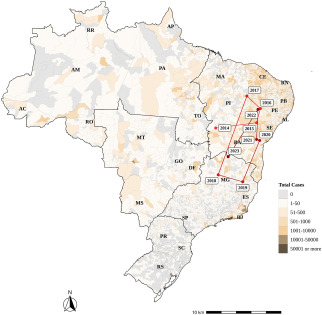
\includegraphics[width=0.6\linewidth]{images/map_cases_brazil}
	\caption{Carte des épicentres des cas de chikungunya chaque année et des cas cumulés par commune jusqu'en 2023~\cite{expansion_chikungunya_brazil}.}
	\label{fig:mapcasesbrazil}
\end{figure}
\newpage
\section{Cas du Paraguay}
Des infections autochtones ont été détectées au \textbf{Paraguay} en 2013, et le CHIKV a été détecté dans le pays chaque année depuis cette date. Sur la base des infections suspectes à CHIKV signalées, le Paraguay a connu quatre vagues épidémiques, en \textbf{2015}, \textbf{2016}, \textbf{2018} et \textbf{2023}, toutes associées aux mois d'été. Du 2 octobre 2022 au 10 avril 2023, un total de \textbf{118 179 }infections suspectes et confirmées ont été signalées, dont\textbf{ 3 510 }cas-patients hospitalisés et 46 décès. En outre, \textbf{294} cas suspects de méningo-encéphalite aiguë ont été signalés, dont \textbf{125} (43\%) ont été attribués au CHIKV ~\cite{giovanetti2023rapid}.
\subsection{Point saillants}
Bien que les températures minimales annuelles soient restées stables au Paraguay au cours des 40 dernières années, les températures moyennes et maximales annuelles ont augmenté régulièrement, et la résurgence rapide et importante du CHIKV en 2022 a coïncidé avec les températures moyennes les plus élevées signalées. Avant 2022, les infections confirmées étaient limitées aux districts de \textit{Central}, \textit{Paraguarí} et \textit{Amambay} (Voir figure \ref{fig:paraguayregioncases}) ; le district de Central dominait les rapports. Après la résurgence virale de 2022, des infections confirmées ont été signalées dans tous les districts.
\begin{figure}[h!]
	\centering
	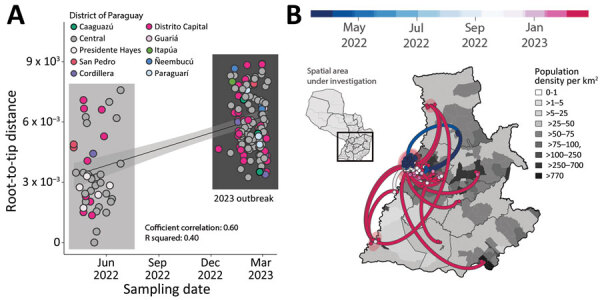
\includegraphics[width=0.8\linewidth]{images/paraguay_region_cases}
	\caption[Expansion de l'épidémie de chikungunya de la lignée Est/Centrale/Sud/Africaine au Paraguay~\cite{rapid_expansion_chikungunya_paraguay}]{A) L'analyse examine les distances génétiques entre les échantillons de virus et leurs dates d'échantillonnage, avec des intervalles de confiance à 90 \%. Les couleurs montrent les lieux d'origine des échantillons. B) La propagation du virus CHIKV ECSA au Paraguay est cartographiée, les cercles indiquant les points clés de la phylogénie, montrant comment le virus s'est diffusé géographiquement au fil du temps~\cite{rapid_expansion_chikungunya_paraguay}.}
	\label{fig:paraguayregioncases}
\end{figure}
\subsection{Contexte}
Cas de chikungunya rapportés chaque semaine (zone grise), incidence normalisée pour \textbf{100 000} personnes (ligne bleue) et \textbf{décès} cumulés voir Figure ~\ref{fig:paraguaycases}.
\begin{figure}[h!]
	\centering
	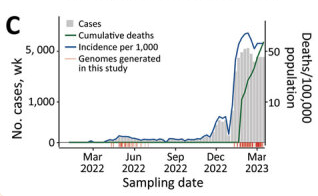
\includegraphics[width=0.8\linewidth]{images/paraguay_cases}
	\caption{Cas de chikungunya déclarés chaque semaine\cite{rapid_expansion_chikungunya_paraguay}}
	\label{fig:paraguaycases}
\end{figure}

\chapter{Revue de la litterature et concepts de base}

\section{Introduction}

\section{Apprentissage Automatique (Machine Learning)}

Bla

\subsection{Concepts de base}

Bla

\subsection{La régression linéaire}

Bla

\subsection{Forêt aléatoire (Random Forest)}

Bla

\section{Apprentissage Profond (Deep Learning)}

Bla

\subsection{Réseaux de neurones profonds}

Bla

\subsection{Algorithmes spécifiques (e.g., LSTM, CNN)}

Bla

\section{Régression par Ensemble}

Bla

\subsection{Concepts de régression par ensemble}

Bla

\subsection{Avantages des méthodes d'ensemble}

Bla

\subsection{Algorithmes d'ensemble (e.g., Gradient Boosting, XGBoost)}

Bla Bla

%\part*{Contribution}

\chapter{Implémentation des Modèles}

\section{Introduction}

\section{Présentation des Outils Utilisés}

Bla

\subsection{Langages et librairies (e.g., Python, Scikit-learn, TensorFlow)}

Bla

\subsection{Infrastructure matérielle (e.g., GPU, serveurs)}

Bla

\section{Méthodes de l'Apprentissage Automatique}

Bla

\subsection{Le jeu de données}

Bla

\subsection{Préparation et nettoyage des données}

Bla

\subsection{Implémentation des modèles de machine learning}

Bla

\section{Méthodes de l'Apprentissage Profond}

Bla

\subsection{Le jeu de données}

Bla

\subsection{Préparation des données pour le deep learning}

Bla

\subsection{Implémentation des modèles de deep learning}

Bla

\chapter{RÉSULTAT ET DISCUSSIONS}
Ce chapitre se concentre sur l’analyse des résultats de prédiction obtenus après l’application des méthodes de machine learning aux données climatiques et aux cas antérieurs de Chikungunya dans trois pays : le \textbf{Tchad}, le \textbf{Brésil} et le \textbf{Paraguay}. L’objectif est de présenter en détail les résultats, de proposer une discussion approfondie, et d’identifier les éventuelles lacunes ou limitations.

\section{Méthode de Validation Croisée (Entraînement et Test)}
L'ensemble de données, composé de 366 instances pour le \textbf{Tchad} et de 1826 instances pour le \textbf{Brésil} et le \textbf{Paraguay}, comprenant des données climatiques et des informations sur les cas de Chikungunya, a été divisé en deux parties pour l’apprentissage. Tout d’abord, les données ont été mélangées, puis elles ont été séparées en deux ensembles : 80 \% des données ont été utilisées pour l’entraînement (ensemble d’apprentissage) et 20 \% ont été réservées pour les tests (ensemble de test).

\section{Choix des Hyperparamètres des Modèles d'Ensemble}
Les hyperparamètres des modèles utilisés pour déterminer leurs performances sont détaillés ci-dessous.

\subsection{Cas du Random Forest Regressor}
Cette section détaille les choix des hyperparamètres spécifiques pour le \textbf{Random Forest Regressor} et leur impact sur la précision des prédictions. Ces hyperparamètres ont été ajustés à l’aide de la méthode de \textbf{recherche en grille} (\textbf{Grid Search}) afin d’optimiser les performances du modèle illustré dans le tableau \ref{tab:grid-search-rf}.

\begin{table}[!hbt]
	\centering
	\caption{Description des hyperparamètres optimisés pour le Random Forest Regressor avec GridSearch}
	\label{tab:grid-search-rf}
	\begin{tabular}{|c|c|c|c|c|}
		\hline
		& \multicolumn{4}{c|}{Hyperparamètres} \\
		\hline
		Pays & \textsf{n\_estimators} & \textsf{max\_depth} & \textsf{min\_samples\_leaf} & \textsf{min\_samples\_split} \\
		\hline
		Tchad & 200 & 10 & 2 & 2 \\
		\hline
		Brésil & 200 & 20 & 2 & 2 \\
		\hline
		Paraguay & 200 & None & 1 & 5 \\
		\hline
	\end{tabular}
\end{table}

Les hyperparamètres utilisés pour le \textbf{Random Forest Regressor} sont les suivants :
\begin{itemize}
	\item \textbf{n\_estimators} : Le nombre d'arbres dans la forêt. Un nombre plus élevé d'arbres peut améliorer la performance, mais augmente aussi le temps de calcul.
	\item \textbf{max\_depth} : La profondeur maximale des arbres. Une profondeur plus grande permet au modèle de capturer plus de complexité, mais risque de surapprendre (overfitting).
	\item \textbf{min\_samples\_leaf} : Le nombre minimum d'échantillons requis pour être dans une feuille. Un nombre plus élevé peut entraîner un modèle plus simple et réduire le surapprentissage.
	\item \textbf{min\_samples\_split} : Le nombre minimum d'échantillons requis pour diviser un nœud interne. Un nombre plus élevé peut rendre le modèle moins sensible au bruit.
\end{itemize}

\subsection{Cas du XGBoost Regressor}
Cette section présente les hyperparamètres choisis pour le \textbf{XGBoost Regressor} et leur impact sur la précision des prédictions. Ces hyperparamètres ont également été ajustés à l’aide de la méthode de \textbf{recherche en grille} (\textbf{Grid Search}) afin d’optimiser les performances du modèle illustré dans le tableau \ref{tab:grid-search-xb}.

\begin{table}[!hbt]
	\centering
	\caption{Description des hyperparamètres optimisés pour le XGBoost Regressor avec GridSearch}
	\label{tab:grid-search-xb}
	\begin{tabular}{|c|c|c|c|c|}
		\hline
		& \multicolumn{4}{c|}{Hyperparamètres} \\
		\hline
		Pays & \textsf{n\_estimators} & \textsf{max\_depth} & \textsf{subsample} & \textsf{learning\_rate} \\
		\hline
		Tchad & 300 & 5 & 0.8 & 0.2 \\
		\hline
		Brésil & 100 & 5 & 1.0 & 0.2 \\
		\hline
		Paraguay & 100 & 7 & 0.1 & 0.2 \\
		\hline
	\end{tabular}
\end{table}

Les hyperparamètres utilisés pour le \textbf{XGBoost Regressor} sont les suivants :
\begin{itemize}
	\item \textbf{n\_estimators} : Le nombre d'arbres dans la forêt.
	\item \textbf{max\_depth} : La profondeur maximale des arbres. Comme pour le Random Forest, une plus grande profondeur peut capturer plus de complexité, mais risque de surapprentissage.
	\item \textbf{subsample} : La proportion d'échantillons utilisés pour entraîner chaque arbre. Une valeur inférieure à 1.0 réduit le surapprentissage en introduisant plus de diversité dans les arbres.
	\item \textsf{learning\_rate} : Le taux d'apprentissage, qui contrôle la contribution de chaque modèle supplémentaire. Un taux plus bas nécessite plus d'estimators pour converger, mais peut conduire à une meilleure généralisation.
\end{itemize}

\section{Résultats obtenus par nos modèles}
Cette section, nous exposons nos résultats à travers un tableau, suivi d’une discussion approfondie. Par la suite, nous illustrons les diverses mesures de performance à l’aide de graphiques variés.
\subsection{Tableau des performance de nos modèles}
Le tableau~\ref{tab:performance} ci-dessous illustre les métriques d’évaluation des résultats de nos travaux.

Les résultats obtenus montrent que le \textit{modèle d'ensemble}, en particulier le \textbf{Voting Regressor}, a globalement surpassé les autres modèles en termes de précision. Il a permis de réduire les erreurs (\textbf{MAE} et \textbf{RMSE}) et d'augmenter le score R\textsuperscript{2}, indiquant une meilleure explication de la variance des données.

Pour le \textbf{Paraguay}, le \textbf{Voting Regressor} a obtenu un RMSE le plus faible (\textbf{68.1025}) et le meilleur score R\textsuperscript{2} (\textbf{0.5957}), surpassant les modèles RandomForestRegressor et XGBoostRegressor.

Au \textbf{Brésil}, bien que le modèle RandomForestRegressor ait montré de très bonnes performances (RMSE de\textbf{ 281.1369} et R\textsuperscript{2} de \textbf{0.9111}), le \textbf{Voting Regressor} a réussi à obtenir des résultats comparables avec un RMSE particulièrement bas de \textbf{163.0350}.

Pour le \textbf{Tchad}, les performances des modèles étaient globalement plus faibles, mais le \textbf{Voting Regressor} a tout de même montré une légère amélioration par rapport aux autres modèles, bien que le score R\textsuperscript{2} reste faible (\textbf{0.3434}).

En conclusion, les modèles d'ensemble, et particulièrement le \textbf{Voting Regressor}, a révélés être les plus performants pour prédire les cas de Chikungunya dans les trois pays étudiés.Toutefois, avec des prédictions plus fiables pour le \textbf{Brésil} et le \textbf{Paraguay} que pour le Tchad, ce qui est dû à la quantité des données disponibles pour ce pays là.

\begin{table}[!hbt]
	\centering
	\caption{Tableau de comparaison des différents modèles}
	\label{tab:performance}
	\begin{tabular}{|c|c|c|c|c|}	
		
		\hline
		Pays & Modèle & MAE & RMSE & R\textsuperscript{2} score \\
		\hline
		\multirow{4}{*}{Paraguay} & LinearRegressor & 65.4165 & 85.5322 & 0.3623 \\
		\cline{2-5}
		& RandomForestRegressor & 38.4501 & 69.9400 & 0.5736 \\
		\cline{2-5}
		& XGBoostRegressor & 40.4713 & 72.3494 & 0.5437 \\
		\cline{2-5}
		& \textbf{VotingRegressor} & \textbf{43.0001} & \textbf{68.1025} & \textbf{0.5957} \\
		\hline
		\multirow{4}{*}{Brésil} & LinearRegressor & 299.0416 & 396.7418 & 0.8229 \\
		\cline{2-5}
		& RandomForestRegressor & 141.0863 & 281.1369 & 0.9111 \\
		\cline{2-5}
		& XGBoostRegressor & 154.3493 & 288.9261 & 0.9061\\
		\cline{2-5}
		& \textbf{VotingRegressor} & \textbf{163.0350}  & \textbf{163.0350} & \textbf{0.9108} \\
		\hline
		\multirow{4}{*}{Tchad} & LinearRegressor & 51.5692 & 90.1886 & 0.1344 \\
		\cline{2-5}
		& RandomForestRegressor & 49.2575 & 79.7674 & 0.3229 \\
		\cline{2-5}
		& XGBoostRegressor & 51.1603 & 80.1259 & 0.3168 \\
		\cline{2-5}
		& \textbf{VotingRegressor} & \textbf{47.6738} & \textbf{78.5506} & \textbf{0.3434} \\
		\hline
	\end{tabular}
\end{table}

\subsection{Performance en RMSE et R2 Score}
La figure \ref{fig:metriccomparaison} montre en termes de RMSE et de coefficient de détermination R2, le niveau de performance de chacun des modèles.
\begin{figure}[h!]
	\centering
	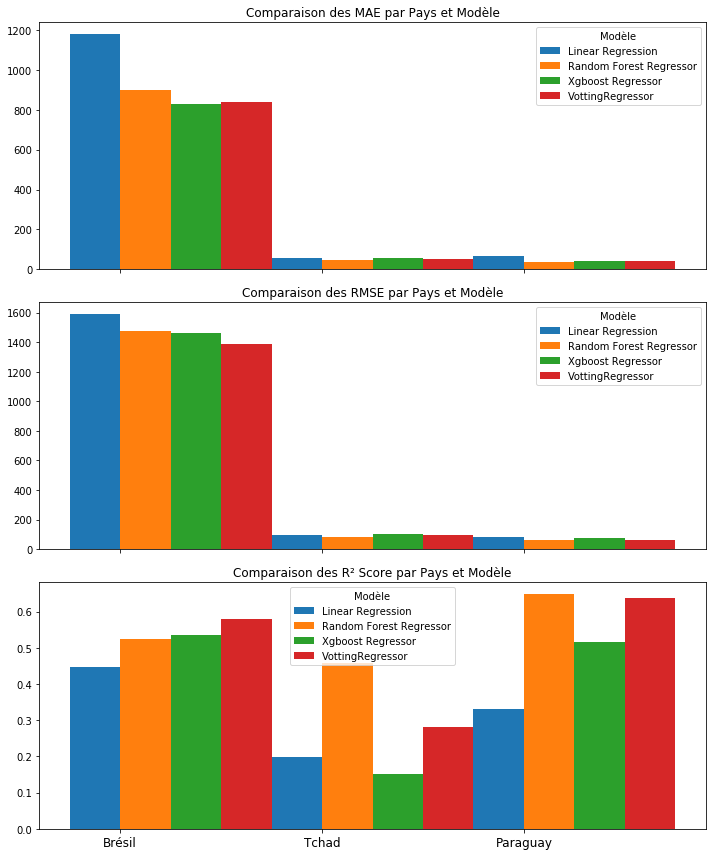
\includegraphics[width=0.8\linewidth]{images/metric_comparaison}
	\caption{Comparaison performance}
	\label{fig:metriccomparaison}
\end{figure}
\newpage
\subsection{Prédiction}
Ci-dessous les prédiction des test dans chaque pays pour le modèle d'ensemble (\textbf{VotingRegressor})
\subsubsection{Pour le Brésil}
La figure \ref{fig:predictionbresil} illustre la phase de prédiction du chikungunya au brésil. 
\begin{figure}[h!]
	\centering
	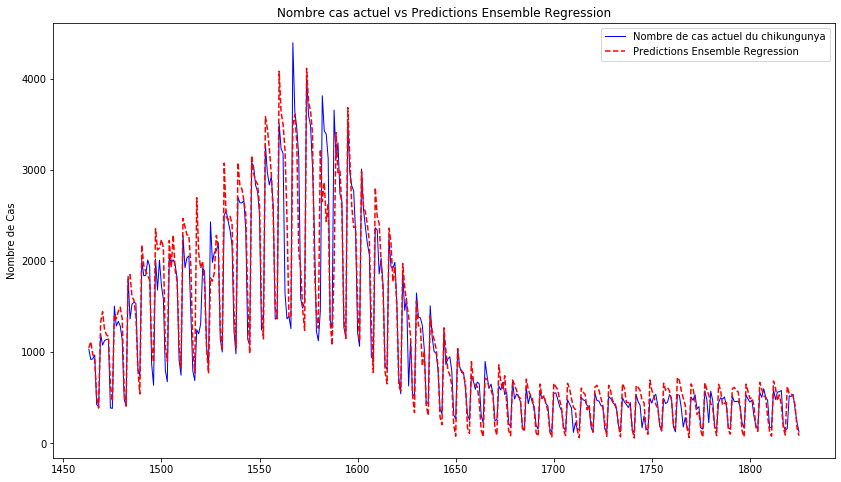
\includegraphics[width=1\linewidth]{images/prediction_bresil}
	\caption{Prédiction Brésil}
	\label{fig:predictionbresil}
\end{figure}

\subsubsection{Pour le Tchad}
La figure \ref{fig:predictionchad} illustre la phase de prédiction du chikungunya au Tchad. 
\begin{figure}[h!]
	\centering
	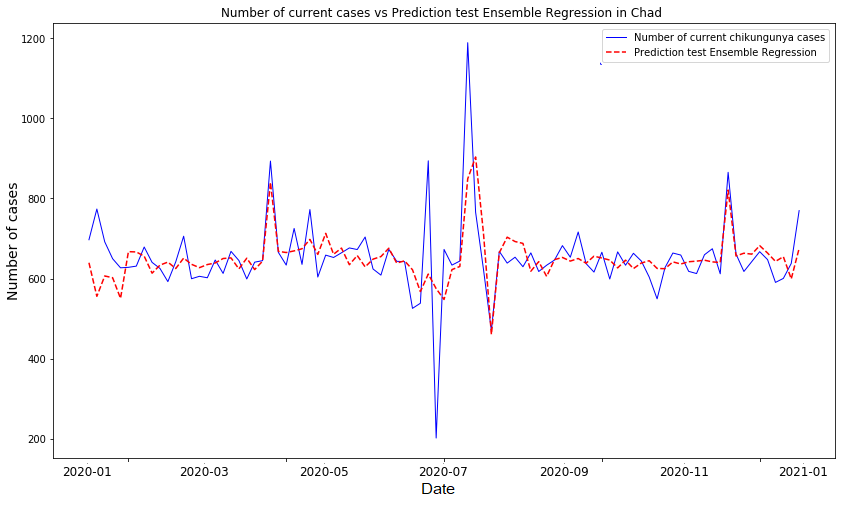
\includegraphics[width=0.85\linewidth]{images/prediction_chad}
	\caption{Prédiction Tchad}
	\label{fig:predictionchad}
\end{figure}
\subsubsection{Pour le Paraguay}
La figure \ref{fig:predictionparaguay} illustre la phase de prédiction du chikungunya au paraguay. 
\begin{figure}[h!]
	\centering
	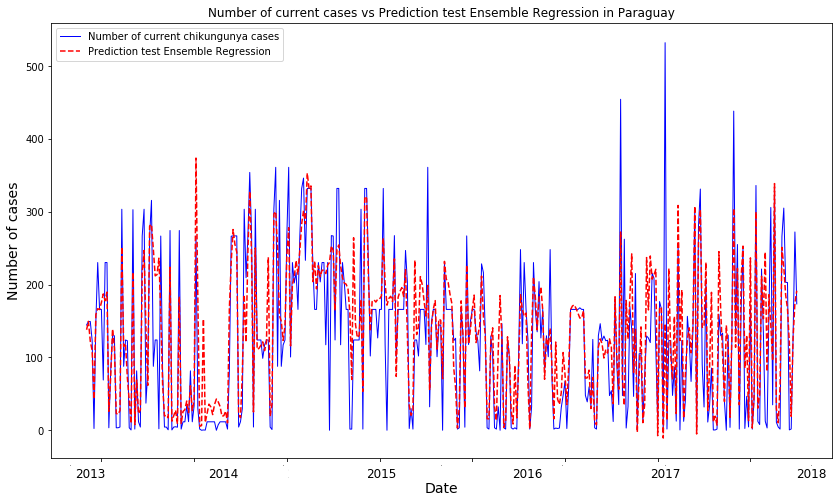
\includegraphics[width=0.85\linewidth]{images/prediction_paraguay}
	\caption{Prédiction Paraguay}
	\label{fig:predictionparaguay}
\end{figure}
\newpage
\section{Discussion}

Les résultats obtenus dans notre étude montrent une performance compétitive des modèles de régression appliqués aux données climatiques et épidémiologiques de la Chikungunya. En particulier, notre modèle d'ensemble \textit{Voting Regressor}, qui combine les prédictions des modèles \textit{Linear Regressor}, \textit{RandomForest Regressor}, et \textit{XGBoost Regressor}, a affiché des performances globalement supérieures aux autres modèles individuels, avec un \textbf{MAE} minimal et un \textbf{RMSE} relativement bas.

Dans le cas du \textbf{Paraguay}, le \textit{Voting Regressor} a atteint un \textbf{MAE} de \textbf{43.00}, soit une amélioration par rapport au \textit{RandomForestRegressor} et au \textit{XGBoostRegressor} qui affichent des \textbf{MAE} respectifs de \textbf{38.45} et \textbf{40.47}. Le RMSE du \textit{Voting Regressor} est de 68.10, indiquant une bonne capacité de prédiction malgré la complexité des données épidémiologiques et climatiques. Le score R² de \textbf{0.5957 }montre que ce modèle explique environ 60 \% de la variance des données pour cette région.

Pour le \textbf{Brésil}, le \textit{Voting Regressor} a montré une robustesse similaire avec un score R² de \textbf{0.9108}, ce qui est légèrement inférieur à celui du \textit{RandomForestRegressor} mais supérieur au \textit{XGBoostRegressor}. Cela suggère que le \textit{Voting Regressor} parvient à combiner les forces de chaque modèle pour fournir des prédictions plus équilibrées, même dans des contextes de données plus hétérogènes.

Au \textbf{Tchad}, bien que les performances générales des modèles soient moins élevées, le \textit{Voting Regressor} reste le modèle le plus performant avec un \textbf{MAE} de \textbf{47.67} et un RMSE de \textbf{78.55}. Le score R² de \textbf{0.3434} est le plus élevé parmi les modèles testés pour cette région, indiquant que ce modèle capture mieux la variance des données malgré des difficultés apparentes liées à la la quantité des données disponibles pour cette région, bien évidement que les techniques de \textbf{data augmentation} et du \textbf{KNNimputer} ont été d'une importance crucial sur ces résultats.

Dans notre contexte, l'imprécision observée dans certaines régions, comme au Tchad, pourrait être due à un manque de prédicteurs ou de variables explicatives dans le modèle, ce qui suggère qu'une exploration plus approfondie des facteurs climatiques et épidémiologiques est nécessaire. De plus, l'impact des variables climatiques telles que la \textbf{température} et l'\textbf{humidité} mérite une attention particulière. Il a été observé, par exemple, qu'une augmentation de la température pourrait être associée à une diminution des cas de Chikungunya, tandis que l'\textbf{humidité} semble accroître ces cas. Ce genre de corrélations, bien que contre-intuitives, pourrait fournir des pistes intéressantes pour affiner les modèles prédictifs.

\part*{Conclusion et perspectives} 
 
\chapter*{Conclusion Générale et perspectives}
\addcontentsline{toc}{chapter}{Conclusion Générale et Perspectives}

L'objectif principal de cette étude était de développer un modèle prédictif du chikungunya, en utilisant des approches de régression d'ensemble issues de l'intelligence artificielle en examinant l'influence des variables climatiques sur la propagation du Chikungunya au Brésil, au Paraguay et au Tchad, en s'appuyant sur des modèles de \textbf{régression avancés}. 

Les données épidémiologiques ont été obtenues sur le site du monitoring des cas d'épidomologie en temps réel PAHO (pour le Paraguay) ,dans le rapport d'OMS(pour le cas du Tchad) et dans le site mendeley pour celui du brésil tandis que les données climatiques provenaient de sources fiables telles que le site WeatherAndClimate.  Les modèles choisis pour cette étude incluaient le \textbf{Random Forest Regressor} et le \textbf{XGBoost Regressor} optimisé via \textbf{Grid Search}, ainsi qu'un modèle d'ensemble (\textbf{Voting Regressor}) combinant \textbf{Linear Regression}, \textbf{Random Forest Regressor} et le \textbf{XGBoost Regressor} optimisé. Parmi ces modèles, notre modèle d'ensemble \textbf{Voting Regressor}, qui combine les prédictions des modèles \textbf{Linear Regression}, \textbf{Random Forest Regressor} et \textbf{XGBoost Regressor}, a affiché des performances globalement supérieures aux autres modèles individuels, avec un \textbf{MAE} minimal, un \textbf{RMSE} relativement bas et une très bonne précision (\textbf{91,08\%} pour le Brésil, \textbf{34,34\%} pour le Tchad et \textbf{59,57\%} pour le Paraguay).

Les limites de l’étude ont montré que les variables climatiques ne suffisent pas à elles seules à expliquer les variations des cas de chikungunya dans ces pays. Il est proposé, pour les futures
recherches, d’intégrer d’autres facteurs environnementaux et de développer un modèle hybride combinant des algorithmes d’apprentissage automatique pour affiner les prévisions. Les recommandations incluent l’amélioration de la collecte des données, l’adoption de stratégies adaptées aux variations climatiques, et la sensibilisation des communautés sur l’hygiène et la prévention
du chikungunya.









% récupérer les citations avec "/footnotemark"
\nocite{*}

% choix du style de la biblio
%\bibliographystyle{plain}
%\addbibresource{bibliographie}
\bibliographystyle{spmpsci}
% inclusion de la biblio
\bibliography{bibliographie}
% voir wiki pour plus d'information sur la syntaxe des entrées d'une bibliographie

%\chapter*{Annexe}
\addcontentsline{toc}{chapter}{Annexe}

\newpage
\end{spacing}{}

\end{document}
